\documentclass{standalone}
\usepackage{tikz}
\usetikzlibrary{patterns, positioning}

\begin{document}
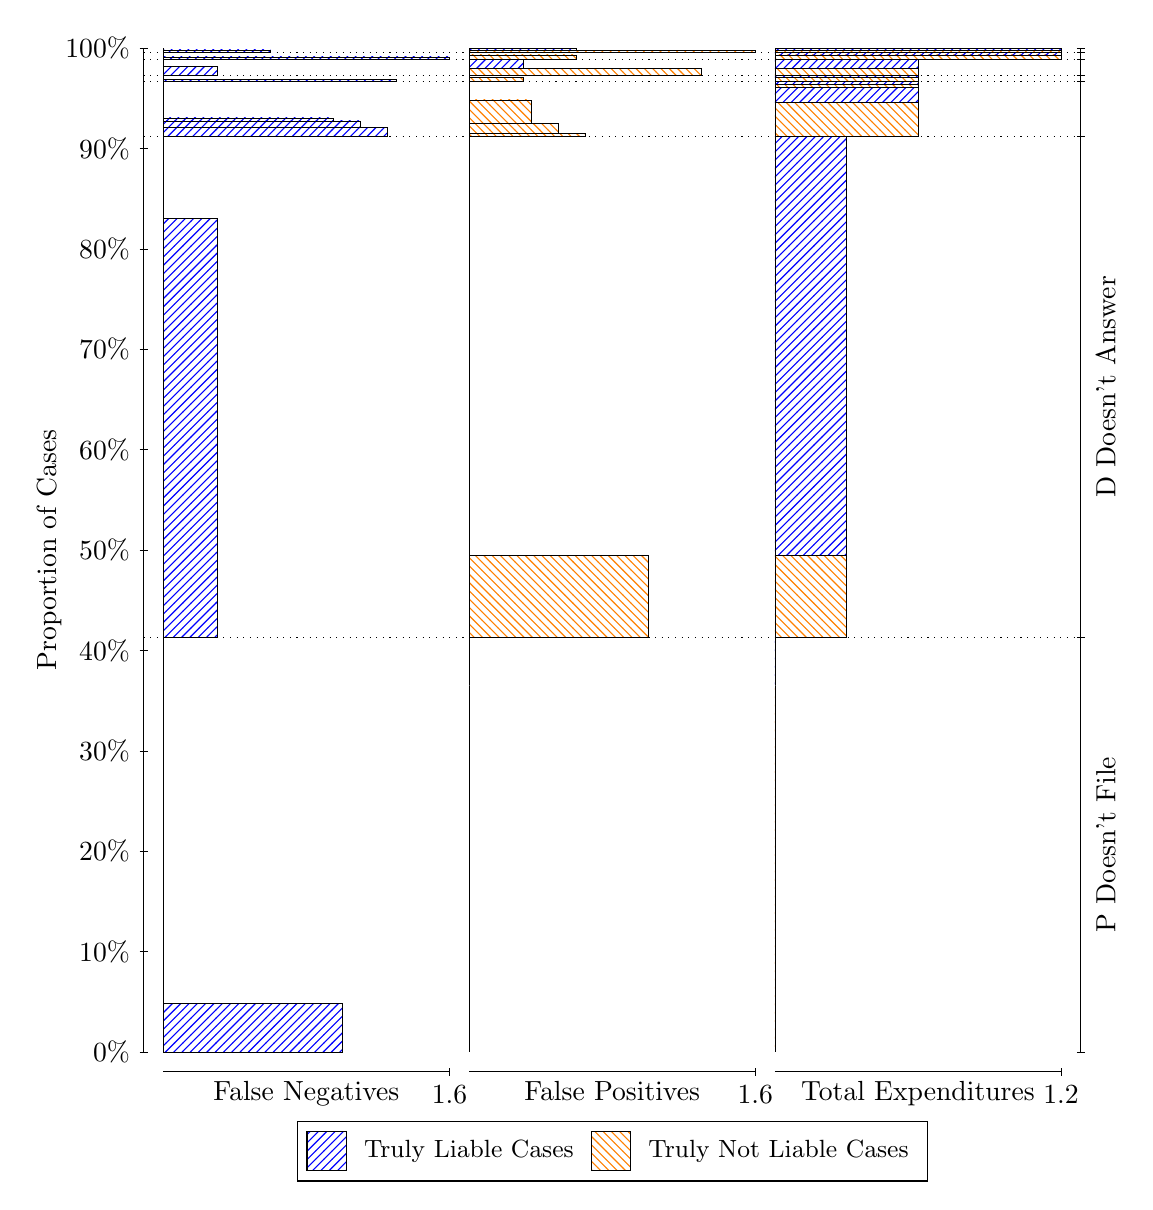
\begin{tikzpicture}
\draw[black, very thin] (1.5,1.75) -- (1.5,14.5);
\node[rotate=90, anchor=center] at (0.3, 8.125) {Proportion of Cases};
\draw[black, very thin] (1.45,1.75) -- (1.55,1.75);
\node[anchor=east] at (1.45, 1.75) {0\%};
\draw[black, very thin] (1.45,3.025) -- (1.55,3.025);
\node[anchor=east] at (1.45, 3.025) {10\%};
\draw[black, very thin] (1.45,4.3) -- (1.55,4.3);
\node[anchor=east] at (1.45, 4.3) {20\%};
\draw[black, very thin] (1.45,5.575) -- (1.55,5.575);
\node[anchor=east] at (1.45, 5.575) {30\%};
\draw[black, very thin] (1.45,6.85) -- (1.55,6.85);
\node[anchor=east] at (1.45, 6.85) {40\%};
\draw[black, very thin] (1.45,8.125) -- (1.55,8.125);
\node[anchor=east] at (1.45, 8.125) {50\%};
\draw[black, very thin] (1.45,9.4) -- (1.55,9.4);
\node[anchor=east] at (1.45, 9.4) {60\%};
\draw[black, very thin] (1.45,10.675) -- (1.55,10.675);
\node[anchor=east] at (1.45, 10.675) {70\%};
\draw[black, very thin] (1.45,11.95) -- (1.55,11.95);
\node[anchor=east] at (1.45, 11.95) {80\%};
\draw[black, very thin] (1.45,13.225) -- (1.55,13.225);
\node[anchor=east] at (1.45, 13.225) {90\%};
\draw[black, very thin] (1.45,14.5) -- (1.55,14.5);
\node[anchor=east] at (1.45, 14.5) {100\%};

\draw[black, very thin] (13.4,1.75) -- (13.4,14.5);
\draw[black, very thin] (13.35,1.75) -- (13.45,1.75);
\node[anchor=west] at (13.35, 1.75) {};
\draw[black, very thin] (13.35,7.0161) -- (13.45,7.0161);
\node[anchor=west] at (13.35, 7.0161) {};
\draw[black, very thin] (13.35,13.378) -- (13.45,13.378);
\node[anchor=west] at (13.35, 13.378) {};
\draw[black, very thin] (13.35,14.077) -- (13.45,14.077);
\node[anchor=west] at (13.35, 14.077) {};
\draw[black, very thin] (13.35,14.151) -- (13.45,14.151);
\node[anchor=west] at (13.35, 14.151) {};
\draw[black, very thin] (13.35,14.356) -- (13.45,14.356);
\node[anchor=west] at (13.35, 14.356) {};
\draw[black, very thin] (13.35,14.446) -- (13.45,14.446);
\node[anchor=west] at (13.35, 14.446) {};
\draw[black, very thin] (13.35,14.5) -- (13.45,14.5);
\node[anchor=west] at (13.35, 14.5) {};

\draw[black, very thin, pattern color=blue, pattern=north east lines] (1.75,1.75) rectangle (4.0208,2.365);
\draw[black, very thin, pattern color=orange, pattern=north west lines] (1.75,2.365) rectangle (1.75,7.0161);
\draw[black, very thin, pattern color=blue, pattern=north east lines] (1.75,7.0161) rectangle (2.4312,12.336);
\draw[black, very thin, pattern color=orange, pattern=north west lines] (1.75,12.336) rectangle (1.75,13.378);
\draw[black, very thin, pattern color=blue, pattern=north east lines] (1.75,13.378) rectangle (4.5885,13.492);
\draw[black, very thin, pattern color=blue, pattern=north east lines] (1.75,13.492) rectangle (4.2479,13.576);
\draw[black, very thin, pattern color=blue, pattern=north east lines] (1.75,13.576) rectangle (3.9073,13.613);
\draw[black, very thin, pattern color=orange, pattern=north west lines] (1.75,13.613) rectangle (1.75,14.077);
\draw[black, very thin, pattern color=blue, pattern=north east lines] (1.75,14.077) rectangle (4.7021,14.105);
\draw[black, very thin, pattern color=orange, pattern=north west lines] (1.75,14.105) rectangle (1.75,14.151);
\draw[black, very thin, pattern color=blue, pattern=north east lines] (1.75,14.151) rectangle (2.4312,14.268);
\draw[black, very thin, pattern color=orange, pattern=north west lines] (1.75,14.268) rectangle (1.75,14.356);
\draw[black, very thin, pattern color=blue, pattern=north east lines] (1.75,14.356) rectangle (5.3833,14.388);
\draw[black, very thin, pattern color=orange, pattern=north west lines] (1.75,14.388) rectangle (1.75,14.446);
\draw[black, very thin, pattern color=blue, pattern=north east lines] (1.75,14.446) rectangle (3.1125,14.475);
\draw[black, very thin, pattern color=orange, pattern=north west lines] (1.75,14.475) rectangle (1.75,14.5);
\draw[black, very thin, pattern color=orange, pattern=north west lines] (5.6333,1.75) rectangle (5.6333,6.4011);
\draw[black, very thin, pattern color=blue, pattern=north east lines] (5.6333,6.4011) rectangle (5.6333,7.0161);
\draw[black, very thin, pattern color=orange, pattern=north west lines] (5.6333,7.0161) rectangle (7.9042,8.0581);
\draw[black, very thin, pattern color=blue, pattern=north east lines] (5.6333,8.0581) rectangle (5.6333,13.378);
\draw[black, very thin, pattern color=orange, pattern=north west lines] (5.6333,13.378) rectangle (7.1094,13.415);
\draw[black, very thin, pattern color=orange, pattern=north west lines] (5.6333,13.415) rectangle (6.7687,13.539);
\draw[black, very thin, pattern color=orange, pattern=north west lines] (5.6333,13.539) rectangle (6.4281,13.842);
\draw[black, very thin, pattern color=blue, pattern=north east lines] (5.6333,13.842) rectangle (5.6333,14.077);
\draw[black, very thin, pattern color=orange, pattern=north west lines] (5.6333,14.077) rectangle (6.3146,14.123);
\draw[black, very thin, pattern color=blue, pattern=north east lines] (5.6333,14.123) rectangle (5.6333,14.151);
\draw[black, very thin, pattern color=orange, pattern=north west lines] (5.6333,14.151) rectangle (8.5854,14.239);
\draw[black, very thin, pattern color=blue, pattern=north east lines] (5.6333,14.239) rectangle (6.3146,14.356);
\draw[black, very thin, pattern color=orange, pattern=north west lines] (5.6333,14.356) rectangle (6.9958,14.414);
\draw[black, very thin, pattern color=blue, pattern=north east lines] (5.6333,14.414) rectangle (5.6333,14.446);
\draw[black, very thin, pattern color=orange, pattern=north west lines] (5.6333,14.446) rectangle (9.2667,14.472);
\draw[black, very thin, pattern color=blue, pattern=north east lines] (5.6333,14.472) rectangle (6.9958,14.5);
\draw[black, very thin, pattern color=orange, pattern=north west lines] (9.5167,1.75) rectangle (9.5167,6.4011);
\draw[black, very thin, pattern color=blue, pattern=north east lines] (9.5167,6.4011) rectangle (9.5167,7.0161);
\draw[black, very thin, pattern color=orange, pattern=north west lines] (9.5167,7.0161) rectangle (10.425,8.0581);
\draw[black, very thin, pattern color=blue, pattern=north east lines] (9.5167,8.0581) rectangle (10.425,13.378);
\draw[black, very thin, pattern color=orange, pattern=north west lines] (9.5167,13.378) rectangle (11.333,13.805);
\draw[black, very thin, pattern color=blue, pattern=north east lines] (9.5167,13.805) rectangle (11.333,14.003);
\draw[black, very thin, pattern color=orange, pattern=north west lines] (9.5167,14.003) rectangle (11.333,14.04);
\draw[black, very thin, pattern color=blue, pattern=north east lines] (9.5167,14.04) rectangle (11.333,14.077);
\draw[black, very thin, pattern color=orange, pattern=north west lines] (9.5167,14.077) rectangle (11.333,14.123);
\draw[black, very thin, pattern color=blue, pattern=north east lines] (9.5167,14.123) rectangle (11.333,14.151);
\draw[black, very thin, pattern color=orange, pattern=north west lines] (9.5167,14.151) rectangle (11.333,14.239);
\draw[black, very thin, pattern color=blue, pattern=north east lines] (9.5167,14.239) rectangle (11.333,14.356);
\draw[black, very thin, pattern color=orange, pattern=north west lines] (9.5167,14.356) rectangle (13.15,14.414);
\draw[black, very thin, pattern color=blue, pattern=north east lines] (9.5167,14.414) rectangle (13.15,14.446);
\draw[black, very thin, pattern color=orange, pattern=north west lines] (9.5167,14.446) rectangle (13.15,14.472);
\draw[black, very thin, pattern color=blue, pattern=north east lines] (9.5167,14.472) rectangle (13.15,14.5);
\draw[black, dotted] (1.5,7.0161) -- (13.4,7.0161);
\draw[black, dotted] (1.5,13.378) -- (13.4,13.378);
\draw[black, dotted] (1.5,14.077) -- (13.4,14.077);
\draw[black, dotted] (1.5,14.151) -- (13.4,14.151);
\draw[black, dotted] (1.5,14.356) -- (13.4,14.356);
\draw[black, dotted] (1.5,14.446) -- (13.4,14.446);
\draw[black, very thin] (1.75,1.5) -- (5.3833,1.5);
\node[anchor=north] at (3.5667, 1.5) {False Negatives};
\draw[black, very thin] (5.3833,1.45) -- (5.3833,1.55);
\node[anchor=north] at (5.3833, 1.45) {1.6};

\draw[black, very thin] (5.6333,1.5) -- (9.2667,1.5);
\node[anchor=north] at (7.45, 1.5) {False Positives};
\draw[black, very thin] (9.2667,1.45) -- (9.2667,1.55);
\node[anchor=north] at (9.2667, 1.45) {1.6};

\draw[black, very thin] (9.5167,1.5) -- (13.15,1.5);
\node[anchor=north] at (11.333, 1.5) {Total Expenditures};
\draw[black, very thin] (13.15,1.45) -- (13.15,1.55);
\node[anchor=north] at (13.15, 1.45) {1.2};

\node[black, centered, rotate=90] at (13.72, 4.3831) {P Doesn't File};
\node[black, centered, rotate=90] at (13.72, 10.197) {D Doesn't Answer};






\draw (7.449999999999999,1.5) node[draw=none] (baseCoordinate) {};
\begin{scope}[align=center]
        \matrix[scale=0.5, draw=black, below=0.5cm of baseCoordinate, nodes={draw}, column sep=0.1cm]{
            \node[rectangle, draw, minimum width=0.5cm, minimum height=0.5cm, pattern=north east lines, pattern color=blue] {}; &
            \node[draw=none, font=\small] (B) {Truly Liable Cases}; &
            \node[rectangle, draw, minimum width=0.5cm, minimum height=0.5cm, pattern=north west lines, pattern color=orange] {}; &
            \node[draw=none, font=\small] (B) {Truly Not Liable Cases}; \\
            };
\end{scope}

\end{tikzpicture}
\end{document}